\chapter{Experiments}
\label{ch:experiments}

\section{Dataset}

We were considering four datasets to conduct our experiments. We also considered using two or more datasets, but in the end we decided to perform all our experiments using the current benchmark dataset, the one that is used by researchers to compare their models and publish their results: The COCO dataset, released by Microsoft in 2014  \citet{Lin2014}. At the moment of writing this report, this is without a doubt the preferred benchmark dataset for the image captioning problem. In addition, there is an online server that automates the evaluation and comparison of submitted results. This server is running 24/7, and results are publicly available, so it is actually an open competition, known as the \href{https://competitions.codalab.org/competitions/3221}{Microsoft COCO Image Captioning Challenge}. 

\begin{figure}[hpt]
	\centering
	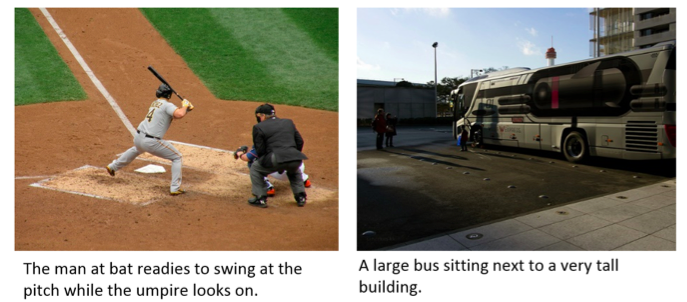
\includegraphics[scale=0.5]{images/ch5/captions-splash.jpg}
	\caption{Image caption examples. Source: \href{http://cocodataset.org/}{COCO Image Captioning Task}}
	\label{fig:caption-example}
\end{figure}


In the end we only used this dataset because the other common options are clearly outdated, such as the Flickr8K and Flickr30K. Although the latter was deemed as an interesting option for faster experiments in the first stages of the project, we finally upgraded the hardware with a very powerfull GPU that made it feasible to use the COCO dataset as the only experimental dataset, and still conduct a considerable number of experiments.

As a matter of fact, there is still a larger dataset supporting image captioning, the Conceptual Captions dataset, by Google  \citep{Sharma2018}, which also offers an online evaluation server and a \href{https://ai.google.com/research/ConceptualCaptions/leaderboard?active_tab=leaderboard}{public leaderboard}. However, it was released just a few months ago, and it is so huge, that it will probably take sometime before it is widely adopted by researchers\footnote{When I started this project there was no results yet but the ones published by google. A month later there are already four additional results from two different teams}.

For our project, we are using the images and the associated captions included in this dataset, which are divided in two separate sets: one for training, and another one for validation purposes.

\subsubsection{Training dataset}

This dataset includes a total of 82,783 unique images which are supposed to have 5 captions each, which would amount to 413,915 captions. However, in fact there are 414,113, probably because some image has more than 5 captions.

The length (number of words) of the captions is highly variable, with a maximum length of 51. The full corpus of text in the training captions dataset is 31,437.

After some initial analysis on the set of captions, we realized that a vast majority of captions are much sorter than the maximum lenght, therefore, for the sake of speeding up the processing of the recurrent layer, we decided to restrict the dataset to those captions having a maximum lenght of 15, which implied removing  13,370 images and 66,885 captions from the training dataset. This filter was applied before tokenizing the captions, thus in practice, when including the "<start>" and "<end>" tokens the maximum length of a sequence would be 17. Note the maximum length of the captions is actually a configurable parameter of the model (\lstinline{config.max_caption_length})

All in all, after filtering the dataset on a maximum caption length basis, we end up with a dataset containing 347,228 instances, each one consisting of a single caption and its associated image.

Concerning the vocabulary, the resulting corpus contains 24,775 words, which is still a huge number, considering than many words only appears once. Finally, we decided to set the vocabulary size to 10,000. The words excluded from the vocabulary were assigned the "<unk>" token. The size of the vocabulary is another hyperparameter of the model (\lstinline{config.vocabulary_size}).



\subsubsection{Validation dataset}

The full validation dataset contains 40504 images and  ???? captions. 
After applying the same filtering schema based on the maximum length of the captions, the dataset was reduced to 34043 images

Note that for the training process, each instance is made up of one single caption and its associated image, whilst for the evaluation process, each instance is an image and all its associated captions. 

\section{Experiments}

For the experiments we trained various models changing some hyperparameters:
\begin{itemize}
    \item The CNN: 'VGG16', 'incept', 'Xception, 'ResNet50', ,'InceptionResNet\_v2'
    \item The Type of units in RNN: 'GRU' or 'LSTM'
    \item The Embedding dimension: 256, 512
    \item The Number of recurrent units: 256, 512
    \item The Number of image features: 256, 512, 1024
    \item The Batchsize: 64, 128
\end{itemize}

We trained all the models for 30 epochs. In one case we trained the model for 90 epochs, but it was clearly overfitted, as 
Unfortunately, due to the long time required to train each model, we were unable to systematically try all the combinations of the chosen hyperparameters. 



\begin{table}[]
\caption{Evaluation results}
\label{tab:results}
\begin{tabular}{lllllllllllllll}
cnn & rnn & embed & state & feat & batch & optimizer & Bleu1 & Bleu2 & Bleu3 & Bleu4 & METEOR & ROUGE & CIDEr & attention \\
incept & lstm & 256 & 512 & 256 & 128 & Adam & 0.510 & 0.337 & 0.213 & 0.131 & 0.164 & 0.364 & 0.410 & False \\
incept & lstm & 256 & 512 & 256 & 64 & Adam & 0.521 & 0.342 & 0.215 & 0.132 & 0.166 & 0.367 & 0.406 & False \\
incept & lstm & 512 & 512 & 256 & 64 & Adam & 0.532 & 0.346 & 0.215 & 0.132 & 0.170 & 0.365 & 0.394 & False \\
incept & gru & 512 & 512 & 512 & 64 & Adam & 0.509 & 0.330 & 0.205 & 0.125 & 0.162 & 0.357 & 0.390 & False \\
incept & gru & 256 & 512 & 256 & 64 & Adam & 0.503 & 0.329 & 0.206 & 0.127 & 0.160 & 0.357 & 0.388 & False \\
incept & gru & 256 & 512 & 256 & 64 & Nadam & 0.515 & 0.336 & 0.209 & 0.127 & 0.163 & 0.360 & 0.380 & False \\
incept & lstm & 256 & 512 & 1024 & 128 & Adam & 0.509 & 0.327 & 0.201 & 0.121 & 0.162 & 0.355 & 0.370 & False \\
xception & gru & 256 & 512 & 256 & 64 & Adam & 0.507 & 0.326 & 0.199 & 0.120 & 0.160 & 0.352 & 0.365 & False \\
incept & gru & 512 & 1024 & 512 & 128 & Adam & 0.490 & 0.314 & 0.192 & 0.116 & 0.155 & 0.347 & 0.355 & False \\
resnet50 & lstm & 256 & 512 & 512 & 128 & Adam & 0.463 & 0.302 & 0.188 & 0.115 & 0.152 & 0.342 & 0.351 & False
\end{tabular}
\end{table}



% 90 epochs overfitting !!

% cnn = inception_v3
% rnn = lstm
% embedding_dim = 512
% rnn_units = 512
% num_features = 512
% weight_initialization = glorot_uniform
% batch_size = 64
% optimizer = Adam

% Final loss after 90 epochs 0.961689

% EPOCH 91 Loss 0.963 ... overfitting

% Bleu_1: 0.489
% Bleu_2: 0.311
% Bleu_3: 0.189
% Bleu_4: 0.113
% METEOR: 0.155
% ROUGE_L: 0.345
% CIDEr: 0.352